\documentclass{article}



\usepackage{arxiv}

\usepackage[utf8]{inputenc} % allow utf-8 input
\usepackage[T1]{fontenc}    % use 8-bit T1 fonts
\usepackage{hyperref}       % hyperlinks
\usepackage{url}            % simple URL typesetting
\usepackage{booktabs}       % professional-quality tables
\usepackage{array}          % ragged-right table columns
\usepackage{float}          % [H] placement for the glossary table
\usepackage{amsfonts}       % blackboard math symbols
\usepackage{amsmath}        % equations
\usepackage{amssymb}
\usepackage{amsthm}         % proposition / proof environments
\usepackage{nicefrac}       % compact symbols for 1/2, etc.
\usepackage{microtype}      % microtypography
\usepackage{lipsum}		% Can be removed after putting your text content
\usepackage{graphicx}
\usepackage{natbib}
\usepackage{doi}

\newtheorem{proposition}{Proposition}
\newcommand{\1}{\mathbf{1}}
\newcommand{\E}{\mathbb{E}}
\newcommand{\RPS}{\mathrm{RPS}}

\title{Forecasting first innings totals of Men's T20 International cricket match}

%\date{September 9, 1985}	% Here you can change the date presented in the paper title
%\date{} 					% Or removing it

\author{
    {\hspace{1mm}Thomas Lee} \\
	% MA in Statistics\\
	University of California, Berkeley\\
	\texttt{tholee@berkeley.edu} \\
    \And
    {\hspace{1mm}Abhishek Shukla} \\
	University of California, Berkeley\\
	\texttt{abhishek.shukla@berkeley.edu} \\
	%% examples of more authors
}

% Uncomment to remove the date
%\date{}

% Uncomment to override  the `A preprint' in the header
\renewcommand{\headeright}{}
\renewcommand{\undertitle}{}
\renewcommand{\shorttitle}{Forecasting T20I first innings totals}

%%% Add PDF metadata to help others organize their library
%%% Once the PDF is generated, you can check the metadata with
%%% $ pdfinfo template.pdf
\hypersetup{
pdftitle={Forecasting first innings totals of Men's T20 International cricket match},
% pdfsubject={q-bio.NC, q-bio.QM},
pdfauthor={Abhishek Shukla, Thomas Lee},
% pdfkeywords={First keyword, Second keyword, More},
}

\begin{document}
\maketitle

\begin{abstract}
We forecast the final first innings total of a men's Twenty20 International (T20I) cricket match while the innings is in progress: before the first ball and after overs 6, 10 and 15. Using ball-by-ball records from Cricsheet, we replay every historical innings and build features only from information available at the moment of the forecast, covering the state of the innings, the players at the crease and still to come, team strength and the venue. Our forecaster is a Bayesian linear regression for the runs still to be scored. We sample from its posterior and posterior predictive distribution and report the forecast as probabilities over 10-run buckets of the final total, so that uncertainty about the model's parameters is carried into the forecast. Forecasts are evaluated with the Ranked Probability Score, which we derive as a sum of Brier scores over over/under thresholds and show to be strictly proper. On test matches from 2024 onward, the model's Ranked Probability Score is 20\% lower than that of an empirical-distribution baseline before the first ball and 70\% lower after 15 overs, and its central 90\% intervals cover 88--92\% of first innings totals.
\end{abstract}


% keywords can be removed
% \keywords{Probabilistic forecasting \and Cricket \and Bayesian linear regression \and Proper scoring rules \and Ranked probability score}


\section{Introduction}
T20 matches are the newest and shortest format of cricket played internationally. Cricket has historically been played over multiple innings, sometimes spanning multiple days. In T20 matches this is brought down to 20 overs (120 balls) for each team and a total of two innings per match. This significantly reduces the duration of a game and has over the years led to its increasing popularity among new fans of the game. But unlike many other sports, cricket is prone to being affected by external factors such as rain or bad light, which may interrupt a match. At present, when a match is interrupted, the target is revised with the Duckworth--Lewis--Stern (DLS) method \citep{duckworth1998,stern2016}. DLS is a static method: it uses a parametric model of the batting ``resources'' (overs and wickets) remaining to set a revised target, and it does not adapt to the teams, players or venue involved. In this project, we build a forecasting model, trained on men's T20 international matches, that forecasts the first innings total of an ongoing match at a given stage.

In-play forecasting in limited-overs cricket has mostly targeted the match result. \citet{bailey2006} predicted the outcome of One-Day Internationals (ODIs) as the game progresses, \citet{asif2016} developed a dynamic logistic regression for in-play win probabilities in ODIs, and \citet{davis2015} built a ball-by-ball simulator for T20 cricket. We instead forecast a full probability distribution over the first innings total, and we evaluate it with a strictly proper scoring rule \citep{gneiting2007}. Readers unfamiliar with cricket can find a short primer on T20 and its key terms in Appendix~\ref{app:primer}.

\section{Data Source}\label{sec:data}
Cricsheet \citep{cricsheet} provides freely available structured data for cricket, including ball-by-ball data from international and T20 league cricket matches and an identifier mapping for the people involved in cricket. In this project we focus only on men's international T20 matches. The only limitation in the coverage of this data is the absence of all games played by the Afghanistan team.\footnote{In November 2024, Cricsheet withdrew all matches featuring Afghanistan's men's team, along with all Afghanistan Premier League matches, in protest at the ICC's treatment of Afghan women's cricketers \citep{cricsheet_afg}, who have been unable to play since the Taliban banned women's sport in 2021. Afghanistan is an ICC full member, so the data lack one of the stronger T20I sides, and the histories of teams that played Afghanistan (their form and Elo ratings) are computed without those matches.}

Each match file contains an \texttt{info} block, with the teams, venue, dates, toss, playing XIs (identified by stable registry IDs) and result, and an \texttt{innings} list in which every delivery records the batter, bowler, non-striker, runs, extras and any wicket. Because every ball is recorded, we can ``forecast the past'' honestly. We replay each historical innings delivery by delivery and compute features using only (i)~the deliveries bowled so far in that innings and (ii)~matches played strictly before the match date.

We keep matches with \texttt{gender} = \texttt{male} and \texttt{team\_type} = \texttt{international}. We use the Cricsheet release whose latest match is dated 9 September 2026, which contains 3{,}539 men's T20Is. We exclude 77 matches that ended with no result and 143 whose first innings was cut short by rain or otherwise curtailed, because their totals are not comparable to full 20-over innings, leaving 3{,}319 matches. No-result matches are still used when computing player, team and venue histories. We treat every T20I as scheduled for 20 overs, because a few Cricsheet files wrongly record 50. Since the ICC granted T20I status to all its member nations in 2019, the data include many matches between associate nations, and the number of matches per year has grown sharply.

\section{Prediction}

\subsection{Outcome}
The outcome is $Y \in \{0, 1, 2, \dots\}$, the final first innings total in runs. We forecast it at four \emph{checkpoints}: before the first delivery (after the toss and team sheets are known), and after overs 6, 10 and 15. These mark the beginning of the match, the end of the powerplay, the halfway point, and the start of the death overs respectively. The checkpoints define four prediction tasks of increasing prior information for the same outcome. A match contributes to a checkpoint only if its first innings reached that point: an innings bowled out in 12.3 overs has no over-15 forecast. Table~\ref{tab:counts} gives the number of innings per checkpoint in each time period (Section~\ref{sec:validation}).

\begin{table}[h]
\centering
\caption{Number of first innings per checkpoint. Train: matches up to 2022; validation: 2023; test: 2024 onward.}
\label{tab:counts}
\begin{tabular}{lrrr}
\toprule
Checkpoint & Train & Validation & Test \\
\midrule
Before ball 1 & 1{,}515 & 331 & 1{,}473 \\
After over 6  & 1{,}515 & 331 & 1{,}473 \\
After over 10 & 1{,}515 & 329 & 1{,}471 \\
After over 15 & 1{,}495 & 324 & 1{,}433 \\
\bottomrule
\end{tabular}
\end{table}

Each forecast is a probability distribution over the final total, reported in buckets of 10 runs: $B_j = \{10j, \dots, 10j + 9\}$ for $j = 0, \dots, 39$, plus a final bucket $B_{40} = \{400, 401, \dots\}$. The forecast assigns a probability $p_j$ to each bucket, with $\sum_j p_j = 1$.

\subsection{Forecasting model: Bayesian linear regression}\label{sec:model}
At a checkpoint where the batting side has scored $s$ runs, we model the runs still to be scored, $R = Y - s$, rather than the total itself. This lets the model concentrate on what remains uncertain. We fit one model per checkpoint, since both the mean and the spread of the remaining runs change sharply as the innings progresses.

\paragraph{Likelihood and prior.} Let $x_i \in \mathbb{R}^p$ be the feature vector of training innings $i$ (Section~\ref{sec:features}), standardized using training-set means and standard deviations and augmented with an intercept, and let $X$ be the $n \times p$ matrix of these vectors, with $r$ the vector of remaining runs. We assume
\begin{equation}
r_i \mid x_i, \beta, \sigma^2 \sim \mathcal{N}(x_i^\top \beta, \sigma^2),
\end{equation}
with the conjugate normal--inverse-gamma prior \citep{bishop2006,gelman2013}
\begin{equation}
\beta \mid \sigma^2 \sim \mathcal{N}(m_0, \sigma^2 V_0), \qquad \sigma^2 \sim \text{Inv-Gamma}(a_0, b_0).
\end{equation}
We center the prior at $m_0 = 0$ with $V_0 = \tau^2 I$, so that $\tau^2$ controls shrinkage of the coefficients (a ridge-type penalty) and is chosen on the validation season. $a_0$ and $b_0$ are small, making the prior on the noise variance weakly informative.

\paragraph{Posterior.} Conjugacy gives the posterior in closed form: $\beta \mid \sigma^2, r \sim \mathcal{N}(m_n, \sigma^2 V_n)$ and $\sigma^2 \mid r \sim \text{Inv-Gamma}(a_n, b_n)$, where
\begin{equation}
\begin{aligned}
V_n &= \big(V_0^{-1} + X^\top X\big)^{-1}, & m_n &= V_n\big(V_0^{-1} m_0 + X^\top r\big), \\
a_n &= a_0 + \tfrac{n}{2}, & b_n &= b_0 + \tfrac12\big(r^\top r + m_0^\top V_0^{-1} m_0 - m_n^\top V_n^{-1} m_n\big).
\end{aligned}
\end{equation}

\paragraph{Sampling the outcome distribution.} For a new innings at the same checkpoint with features $\tilde x$ and current score $s$, we draw $S$ samples. For $k = 1, \dots, S$:
\begin{enumerate}
\item draw $\sigma^{2(k)} \sim \text{Inv-Gamma}(a_n, b_n)$ and $\beta^{(k)} \sim \mathcal{N}(m_n, \sigma^{2(k)} V_n)$ from the posterior;
\item draw the remaining runs $\tilde r^{(k)} \sim \mathcal{N}(\tilde x^\top \beta^{(k)}, \sigma^{2(k)})$ from the likelihood;
\item set the simulated total $\tilde y^{(k)} = s + \max\big(0, \operatorname{round}(\tilde r^{(k)})\big)$, since a total cannot fall below the current score.
\end{enumerate}
The bucket probabilities are the fractions of simulated totals that fall in each bucket:
\begin{equation}
\hat p_j = \frac{1}{S} \sum_{k=1}^{S} \1\{\tilde y^{(k)} \in B_j\}, \qquad j = 0, \dots, 40.
\end{equation}
Step 1 carries uncertainty about the parameters into the forecast, and step 2 adds the ball-to-ball randomness of the innings. The forecast distribution therefore widens for innings whose features are unlike most of the training data. In our implementation we compute the limit of this procedure as $S \to \infty$ exactly rather than by drawing samples, and a unit test confirms that the two agree (Section~\ref{sec:demo}).

\paragraph{From buckets to a CDF.} To score the forecast with the Ranked Probability Score of Section~\ref{sec:scoring}, which is defined on integer totals, we spread each bucket's probability uniformly over its ten totals. For $t = 0, \dots, 399$ this gives
\begin{equation}\label{eq:bucketcdf}
F(t) = \sum_{j < \lfloor t/10 \rfloor} \hat p_j \;+\; \frac{(t \bmod 10) + 1}{10}\, \hat p_{\lfloor t/10 \rfloor},
\end{equation}
and $F(400) = 1$.

\paragraph{Limitations of the model.} A Gaussian likelihood is a simplification: remaining runs are nonnegative integers and can be skewed, especially late in the innings when a collapse is possible. Fitting separate models per checkpoint lets the noise variance vary with the stage of the innings, but within a checkpoint the variance is assumed constant. The model is also linear in its features, so nonlinear effects, such as the interaction between wickets in hand and balls remaining, would have to be supplied as explicit features; we do not add such interaction terms.

\section{Features}\label{sec:features}
We started from a list of candidate features covering the match state, bowling, batting, fielding, venue, recent performance, toss and weather. We kept those that are both predictive in principle and computable from Cricsheet at the moment of the forecast (Table~\ref{tab:features}). All historical aggregates use only matches before the forecast date. Ratings for teams and venues with little history are shrunk toward the global mean, and the number of prior matches is included as a feature so the model can learn how much to trust each rating.

\begin{table}[h]
\centering
\caption{Feature groups (representative feature names in \texttt{typewriter} font).}
\label{tab:features}
\small
\begin{tabular}{>{\raggedright\arraybackslash}p{0.2\linewidth}>{\raggedright\arraybackslash}p{0.73\linewidth}}
\toprule
Group & Features \\
\midrule
Match state & \texttt{score}, \texttt{wickets}, balls remaining, \texttt{run\_rate\_last\_5}, current partnership. The over is fixed at each checkpoint. \\
Batters at the crease & Runs and strike rate so far in this innings, and career T20I average and strike rate, for the striker and non-striker. \\
Batting resources & \texttt{remaining\_batting\_order\_sr}, \texttt{remaining\_batting\_order\_avg}: career T20I strength of the batters yet to bat (the whole XI before ball 1). \\
Bowling resources & \texttt{remaining\_bowling\_economy\_weighted}: career economy rates of the bowling side, weighted by each bowler's remaining overs (at most four per bowler). \\
Team strength & Point-in-time Elo ratings \citep{elo1978} for both sides and their difference, with match counts; recent batting and bowling form (exponentially weighted); team tier (ICC full member or associate). \\
Venue & \texttt{venue\_avg\_first\_innings\_score} (shrunk toward the global mean), \texttt{venue\_n\_prior\_matches}, and whether the batting side is at home, away or at a neutral venue. \\
\bottomrule
\end{tabular}
\end{table}

\paragraph{Excluded features.} We dropped head-to-head records, since most pairs of teams have met too few times for a stable estimate. We dropped toss-based win records, because they measure match results rather than first innings totals. Boundaries and extras so far are already included in the score. Weather, dew, day/night scheduling and pitch reports are plausibly important but are not in Cricsheet.

\section{Validation}\label{sec:validation}
We evaluate forecasts by backtesting on data split by match date: innings from 2022 and earlier are used for training, 2023 for validation (choosing the prior scale $\tau^2$), and 2024 onward for testing. A random split would let information from later matches, such as a team's form or a player's rating, leak into the training set. For the same reason, every feature is computed only from matches before the forecast date, and we test this directly: the features for a match on date $D$ must be unchanged when all matches on or after $D$ are deleted from the history.

\subsection{Scoring Rule}\label{sec:scoring}
A forecast of a total is used to answer threshold questions: will the team score at most $t$ runs? For a single threshold, the natural score is the Brier score \citep{brier1950} of the binary event $\{Y \le t\}$, whose forecast probability is $F(t)$. Summing over all thresholds gives the Ranked Probability Score \citep{epstein1969}, the discrete form of the continuous ranked probability score \citep{matheson1976,gneiting2007}:
\begin{equation}\label{eq:rps}
\RPS(F, y) = \sum_{t=0}^{T} \big(F(t) - \1\{y \le t\}\big)^2, \qquad T = 400.
\end{equation}
Lower is better. If $F$ is a point mass at $\hat y$, then $\RPS(F, y) = |\hat y - y|$, so the score is measured in runs and generalizes absolute error to distributions. For our bucketed forecasts, $F$ is given by Eq.~\eqref{eq:bucketcdf}.

\begin{proposition}[Strict propriety]
Let $Y \sim G$. Then $\E_{Y \sim G}\,\RPS(F, Y)$ is uniquely minimized over CDFs on $\{0, \dots, T\}$ by $F = G$ on $\{0, \dots, T\}$.
\end{proposition}
\begin{proof}
Fix $t$ and write $Z_t = \1\{Y \le t\}$, a Bernoulli variable with mean $G(t)$ and variance $G(t)(1 - G(t))$. Then $\E\,(F(t) - Z_t)^2 = (F(t) - G(t))^2 + \mathrm{Var}(Z_t)$. Summing over $t$,
\begin{equation}\label{eq:decomp}
\E_{Y \sim G}\,\RPS(F, Y) = \sum_{t=0}^{T} \big(F(t) - G(t)\big)^2 \;+\; \sum_{t=0}^{T} G(t)\big(1 - G(t)\big).
\end{equation}
The second sum does not depend on $F$, and the first is nonnegative and equals zero if and only if $F(t) = G(t)$ for every $t$.
\end{proof}

A forecaster who believes $G$ therefore has no incentive to report anything else, which is the property we need to compare forecasters honestly. We prefer RPS to the logarithmic score for three reasons. It rewards being close: forecasting 170 when the outcome is 172 scores far better than forecasting 220, whereas the log score depends only on the probability assigned to exactly 172. It is bounded, so one surprising total does not dominate the average. And it is measured in runs, which is easy to interpret. We report the mean RPS over test innings and the skill score $1 - \overline{\RPS} / \overline{\RPS}_{\text{ECDF}}$ relative to an ECDF baseline, which forecasts every innings with the empirical cumulative distribution function (ECDF) of first innings totals in the training data, bucketed like the model's forecasts, and ignores the teams, venue and state of the innings. We set $T = 400$, above the highest first innings total in our data, so no outcome falls beyond the grid. A total above 400 would incur a small penalty at $t = 400$ under every forecast; this would be a property of the truncated grid, not of the rule, and would affect all forecasters equally.

\subsection{Log Score and Squared Error}\label{sec:otherscores}
We also report two familiar scores, one for the bucket probabilities and one for a single best estimate.

\paragraph{Log score and cross-entropy.} The logarithmic score \citep{gneiting2007} of a bucketed forecast is the negative log probability of the bucket that occurs,
\begin{equation}\label{eq:log}
\mathrm{LS}(p, y) = -\log p_{j(y)}, \qquad j(y) = \min\big(\lfloor y/10 \rfloor, 40\big),
\end{equation}
measured in nats. Averaged over innings, it is the negative log-likelihood of the observed buckets under the forecasts. If the true bucket probabilities are $g = (g_0, \dots, g_{40})$, the expected log score is the \emph{cross-entropy} of $p$ relative to $g$, which splits into the Shannon entropy of $g$ and the Kullback--Leibler (KL) divergence from $g$ to $p$:
\begin{equation}\label{eq:crossent}
\E_{Y \sim G}\,\mathrm{LS}(p, Y) = -\sum_{j} g_j \log p_j = \underbrace{-\sum_{j} g_j \log g_j}_{H(g)} \;+\; \underbrace{\sum_{j} g_j \log \frac{g_j}{p_j}}_{\mathrm{KL}(g \,\|\, p)}.
\end{equation}
The entropy $H(g)$ does not depend on the forecast, and $\mathrm{KL}(g \,\|\, p) \ge 0$ with equality if and only if $p = g$ (Gibbs' inequality), so the log score is strictly proper on buckets. Unlike RPS, it is unbounded: a forecast that gives the realized bucket a probability near zero receives a very large penalty, and a probability of exactly zero gives an infinite score. A forecaster scored this way must give every bucket that can occur positive probability.

\paragraph{Squared error for the best estimate.} The regression part of the forecast is a single best estimate $\hat y$ of the total. We score it by the squared error $(y - \hat y)^2$ and report its mean over test innings (MSE). If $Y \sim G$ has mean $\mu_G$ and variance $\mathrm{Var}_G(Y)$, then
\begin{equation}\label{eq:se}
\E_{Y \sim G}\,(Y - \hat y)^2 = (\hat y - \mu_G)^2 + \mathrm{Var}_G(Y),
\end{equation}
so the expected squared error is minimized by the mean $\hat y = \mu_G$. It is a proper score for the mean, but it ignores the rest of the forecast distribution. By contrast, RPS scores a point forecast by its absolute error, which the median minimizes.

\section{Trial Prediction}\label{sec:trial}
\subsection{Optimal Score}\label{sec:optimal}
Eqs.~\eqref{eq:decomp}, \eqref{eq:crossent} and \eqref{eq:se} share one structure \citep{gneiting2007}. The expected score of a forecast is an \emph{entropy} term, which depends only on the true distribution $G$, plus a \emph{divergence} term, which is nonnegative and zero only for the ideal forecast:
\begin{equation}\label{eq:entdiv}
\E_{Y \sim G}\, S(F, Y) = H_S(G) + d_S(F, G).
\end{equation}
Table~\ref{tab:entropy} lists the pairs for our three scores. The entropy $H_S(G) = \E_{Y \sim G}\, S(G, Y)$ is the expected score of a forecaster who knows $G$ exactly, so it is the optimal score. It is not zero. For RPS, each threshold $t$ is a Bernoulli event $\{Y \le t\}$ that contributes its variance $G(t)(1 - G(t))$ even to the perfect forecast, and this term is positive at every $t$ from the lowest possible total up to, but not including, the highest. Likewise $H(g) > 0$ unless one bucket is certain, and $\mathrm{Var}_G(Y) > 0$ unless the total is. Only a forecaster facing a certain outcome can have an expected score of zero.

\begin{table}[h]
\centering
\caption{Entropy (optimal expected score) and divergence (excess over the optimum) of each score, for a forecast $F$ with bucket probabilities $p$ and best estimate $\hat y$, when $Y \sim G$ with bucket probabilities $g$.}
\label{tab:entropy}
\begin{tabular}{llll}
\toprule
Score & $S(F, y)$ & Entropy $H_S(G)$ (optimum) & Divergence $d_S(F, G)$ \\
\midrule
RPS & $\sum_t \big(F(t) - \1\{y \le t\}\big)^2$ & $\sum_t G(t)\big(1 - G(t)\big)$ & $\sum_t \big(F(t) - G(t)\big)^2$ \\
Log score & $-\log p_{j(y)}$ & $H(g) = -\sum_j g_j \log g_j$ & $\mathrm{KL}(g \,\|\, p)$ \\
Squared error & $(y - \hat y)^2$ & $\mathrm{Var}_G(Y)$ & $(\hat y - \mu_G)^2$ \\
\bottomrule
\end{tabular}
\end{table}

\paragraph{Conditioning on features.} At a checkpoint the forecaster knows the features $x$, so the relevant truth is the conditional distribution $G(\cdot \mid x)$, and the best achievable average score is the Bayes risk $R_S^* = \E_X\, H_S\big(G(\cdot \mid X)\big)$. More information cannot increase it. Each entropy is a minimum of functions that are linear in $G$, $H_S(G) = \min_F \E_{Y \sim G}\, S(F, Y)$, so it is concave. Since $G = \E_X\, G(\cdot \mid X)$, Jensen's inequality gives
\begin{equation}\label{eq:jensen}
R_S^* = \E_X\, H_S\big(G(\cdot \mid X)\big) \;\le\; H_S\big(\E_X\, G(\cdot \mid X)\big) = H_S(G).
\end{equation}
The gap $H_S(G) - R_S^*$ is the value of the features. $R_S^*$ itself is the randomness in the rest of the innings that no forecaster using these features can remove.

\paragraph{Estimating the optimum.} $G(\cdot \mid x)$ is unknown, so $R_S^*$ cannot be computed exactly. We report two estimates in Section~\ref{sec:demo}.
\begin{enumerate}
\item \emph{No features.} Plugging the empirical distribution of the test totals, bucketed like the model's forecasts, into $H_S$ gives the optimal score of a forecaster that gives every innings the same distribution, even one that knew the test-period distribution in advance. By Eq.~\eqref{eq:jensen}, it is an upper bound on $R_S^*$, up to sampling error.
\item \emph{Model-implied.} If the Bayesian model's forecast $\hat F_i$ for test innings $i$ were the truth, its expected score would be $H_S(\hat F_i)$. The average $\frac1n \sum_i H_S(\hat F_i)$ over test innings is therefore the model's own estimate of $R_S^*$. For RPS we use the bucketed CDF of Eq.~\eqref{eq:bucketcdf}, and for squared error we use the predictive variance of $s + \tilde r$, before rounding and truncation.
\end{enumerate}
If the model is correct, its realized mean score should match estimate 2 up to sampling error. A realized score above it means that the forecasts are too narrow or biased, and a realized score below it means that they are too wide.

\subsection{Demo}\label{sec:demo}
\paragraph{Setup.} We fit the model of Section~\ref{sec:model} separately at each checkpoint on the training innings, with the features of Table~\ref{tab:features}: \texttt{score}, \texttt{wickets}, \texttt{run\_rate\_last\_5} and the current partnership; the runs, strike rate and career T20I average and strike rate of both batters at the crease; the batting and bowling resources; both Elo ratings, their difference and both match counts; both teams' recent form; the venue average and number of prior matches; and one-hot indicators for the two team tiers and for home, away or neutral. Features that are constant or missing at a checkpoint drop out: balls remaining at every checkpoint, and the in-play features before ball 1. This leaves 19 features before ball 1 and 31 afterward. Other missing values, mostly career statistics of batters with no previous T20I (6--9\% of batters at the crease across all splits), are set to the training mean. The Elo difference is collinear with the two ratings, and the one-hot indicators with the intercept, but the prior keeps the posterior proper. We set $a_0 = b_0 = 0.01$ and choose $\tau^2 \in \{10^{-3}, 10^{-2}, \dots, 10\}$ by mean validation RPS. The value $\tau^2 = 0.1$ is chosen at every checkpoint. The experiment is reproduced by \texttt{python -m src.experiments.blr}.

\paragraph{Exact bucket probabilities.} Rather than drawing samples, we compute the bucket probabilities exactly: averaging over the posterior gives the predictive distribution of the remaining runs $\tilde r$ in closed form, so its CDF can be evaluated directly. The rounding and truncation in step 3 of Section~\ref{sec:model} are a fixed function of $\tilde r$, and since $t - s \ge 0$, $\max\big(0, \operatorname{round}(\tilde r)\big) \le t - s$ if and only if $\tilde r < t - s + \tfrac12$. So for integer $t \ge s$,
\begin{equation}\label{eq:tcdf}
P(\tilde Y \le t) = P\big(\tilde r < t - s + \tfrac12\big),
\end{equation}
and $P(\tilde Y \le t) = 0$ for $t < s$. The bucket probabilities are $\hat p_j = P(\tilde Y \le 10j + 9) - P(\tilde Y \le 10j - 1)$ for $j = 0, \dots, 39$, and $\hat p_{40} = 1 - P(\tilde Y \le 399)$. This is the limit of the sampler as $S \to \infty$. In a unit test on synthetic data, the two agree to within 0.005 in every bucket with $S = 400{,}000$ draws, including a case where the truncation at $s$ matters. Every bucket the total can still reach receives positive probability, as the log score requires.

\paragraph{Best estimate.} The best estimate is $\hat y = s + \tilde x^\top m_n$, the predictive mean of $s + \tilde r$ before rounding and truncation, which (up to that approximation) minimizes the expected squared error by Eq.~\eqref{eq:se}. We report it together with its bucket $B_{j(\operatorname{round}(\hat y))}$ and that bucket's probability. Because the predictive distribution is symmetric and unimodal, the bucket containing the rounded mean is also the most probable bucket, apart from the truncation at $s$.

\paragraph{Worked example.} Figure~\ref{fig:demo} shows the forecasts for the final of the 2024 ICC Men's T20 World Cup between India and South Africa at Kensington Oval, Bridgetown, a match in the test period. India batted first and made 176/7. Before ball 1 the best estimate is 177, in the 170--179 bucket, which the model gives probability 0.11. India lost three wickets in the powerplay and were 45/3 after six overs. The estimate fell to 164 (bucket 160--169, probability 0.15), and the bucket of the actual total kept probability 0.14. After ten overs (75/3) the estimate was 169, and after fifteen overs (118/4) it was 172, back in the 170--179 bucket, now with probability 0.28. The distribution narrows as the innings progresses and fewer runs remain uncertain.

\begin{figure}[t]
\centering
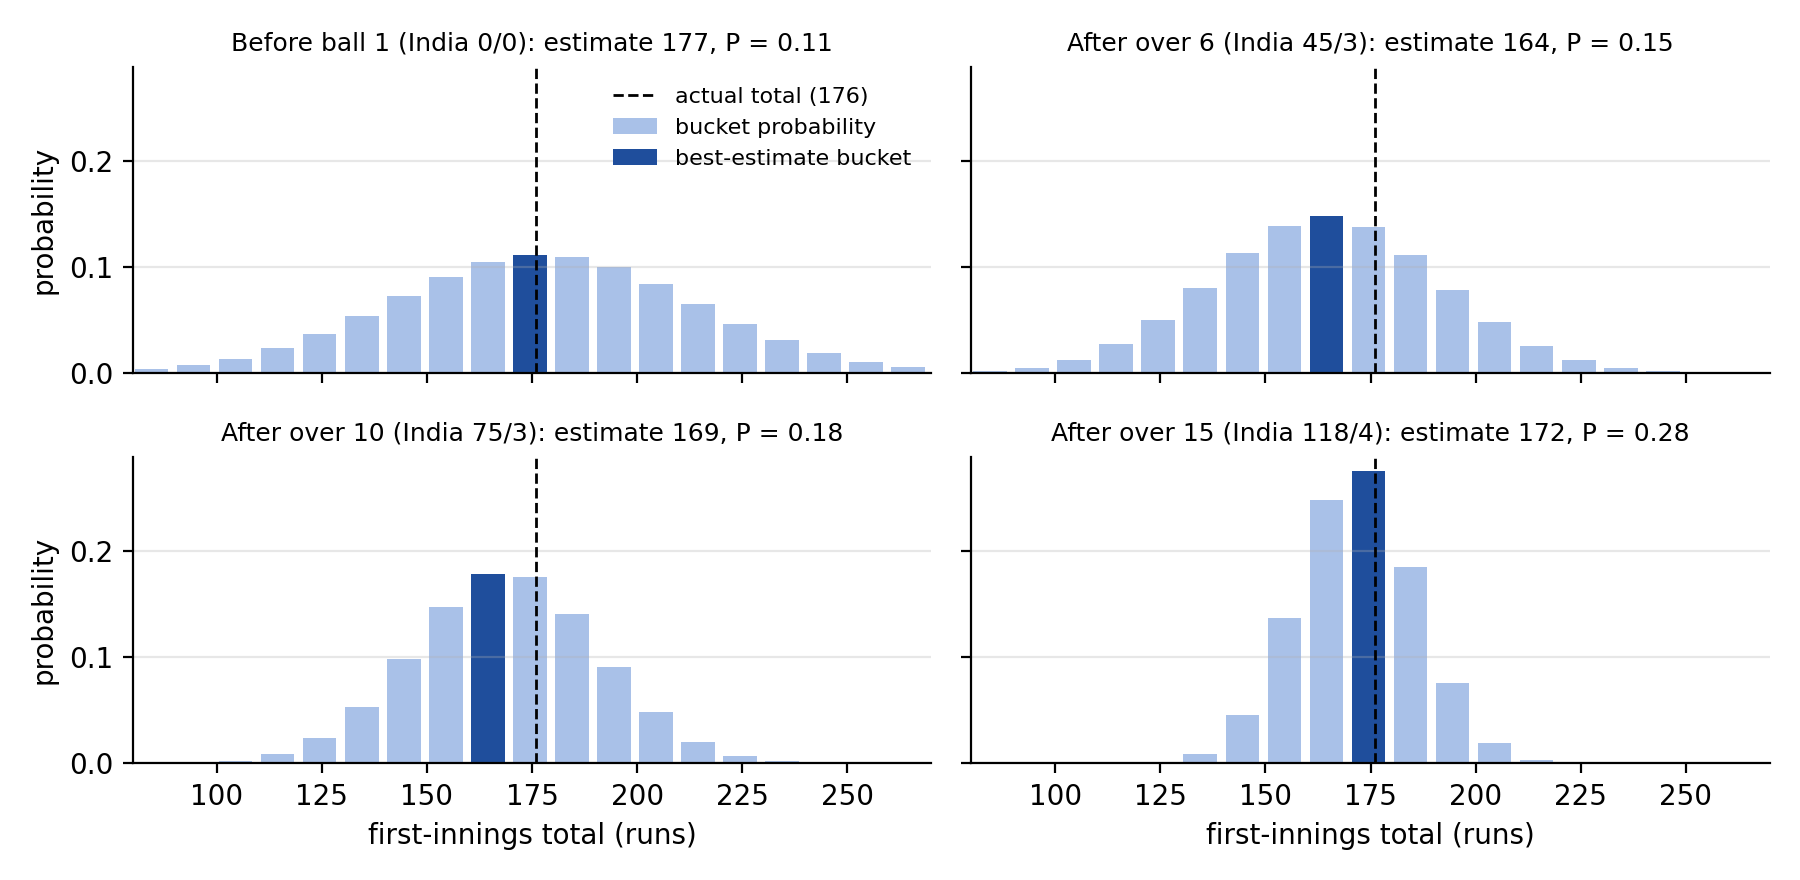
\includegraphics[width=0.9\linewidth]{figs/blr_demo.png}
\caption{Bucket probabilities of the Bayesian linear regression for India's innings in the 2024 T20 World Cup final, at each checkpoint. The dark bar is the bucket of the best estimate $\hat y$, and the dashed line is the actual total of 176.}
\label{fig:demo}
\end{figure}

\paragraph{Test results.} Table~\ref{tab:demo} summarizes the forecasts for all test innings. The model beats the ECDF baseline in RPS by 20\% before ball 1 and by 70\% after over 15. Features lower the optimal score sharply: before ball 1, the model-implied optimal RPS is 20.2 runs, against 26.4 for the best forecast without features, and after over 15 it is 8.1 against 25.1. The optimum is still far from zero. Even after 15 overs, the model expects a perfect forecaster to score about 8 runs of RPS, with a root mean squared error of about 14 runs, because the last five overs remain genuinely uncertain.

\begin{table}[t]
\centering
\caption{Test performance of the Bayesian linear regression (BLR) and estimates of the optimal score (Section~\ref{sec:optimal}). Lower is better for RPS, log score and MSE. RPS is shown $\pm$ one standard error. ``No features'' is the entropy of the empirical distribution of test totals, bucketed like the BLR forecasts. ``Model-implied'' is the expected score if the BLR forecasts were the truth. The ECDF baseline is also bucketed like the BLR forecasts.}
\label{tab:demo}
\small
\begin{tabular}{lcccc}
\toprule
 & Before ball 1 & After over 6 & After over 10 & After over 15 \\
\midrule
\multicolumn{5}{l}{\emph{RPS (runs)}} \\
\quad ECDF baseline & 26.57 & 26.57 & 26.46 & 25.22 \\
\quad BLR & 21.24 {\scriptsize $\pm$ 0.44} & 15.13 {\scriptsize $\pm$ 0.31} & 11.80 {\scriptsize $\pm$ 0.23} & 7.62 {\scriptsize $\pm$ 0.14} \\
\quad Skill vs.\ ECDF baseline & 0.20 & 0.43 & 0.55 & 0.70 \\
\quad Optimum, no features & 26.35 & 26.35 & 26.26 & 25.08 \\
\quad Optimum, model-implied & 20.15 & 15.27 & 12.45 & 8.14 \\
\midrule
\multicolumn{5}{l}{\emph{Log score (nats)}} \\
\quad BLR & 2.76 & 2.42 & 2.17 & 1.73 \\
\quad Optimum, no features & 2.95 & 2.95 & 2.94 & 2.90 \\
\quad Optimum, model-implied & 2.69 & 2.41 & 2.20 & 1.76 \\
\midrule
\multicolumn{5}{l}{\emph{MSE of the best estimate (runs$^2$)}} \\
\quad BLR & 1{,}447 & 738 & 444 & 182 \\
\quad Optimum, no features & 2{,}210 & 2{,}210 & 2{,}193 & 1{,}992 \\
\quad Optimum, model-implied & 1{,}260 & 718 & 473 & 193 \\
\midrule
\multicolumn{5}{l}{\emph{Best estimate and calibration}} \\
\quad Mean error $y - \hat y$ (runs) & $+4.6$ & $+0.7$ & $-1.1$ & $-1.0$ \\
\quad Bucket of $\hat y$ contains $y$ & 0.11 & 0.17 & 0.19 & 0.27 \\
\quad \quad model-implied & 0.11 & 0.15 & 0.18 & 0.28 \\
\quad Coverage of central 90\% interval & 0.88 & 0.90 & 0.91 & 0.92 \\
\bottomrule
\end{tabular}
\end{table}

\paragraph{Distance to the optimum.} Before ball 1, the realized scores exceed the model-implied optimum for all three scores (RPS 21.2 against 20.2, MSE 1{,}447 against 1{,}260), and the model underpredicts test totals by 4.6 runs on average. The average test total is not higher than in training, because the test period has more associate matches, but teams of the same tier scored more: full members averaged 175 runs against 162 in training, and associates 144 against 141. The pre-match features cannot see this shift. About 1 run of the gap comes from the prior shrinking the intercept toward zero, since $V_0 = \tau^2 I$ also covers the intercept. Once the current score is known, it absorbs most of this shift. From over 6 onward, the realized scores are within 7\% of the model-implied values, and after overs 10 and 15 they are slightly below them. The forecasts are then, if anything, slightly too wide, and their central 90\% intervals cover 91--92\% of test totals.

\paragraph{Best estimate and log score.} The bucket of the best estimate contains the actual total in 11\% of test innings before ball 1 and 27\% after over 15, matching the model's own expectation. A 10-run bucket is narrow compared with the forecast error (a root mean squared error of 38 runs before ball 1), so the bucket probabilities carry more information than the single best estimate. The log score shows why a bounded score is safer. Fifteen test totals exceed the highest training total of 263. The ECDF baseline gives their buckets probability zero, as it does the buckets of a few unusually low totals: 19 test innings in all before over 15, and 27 after it. Its log score is therefore infinite, and Table~\ref{tab:demo} reports none. The BLR forecasts give every reachable bucket positive probability, but a single surprising innings still costs up to 12.6 nats, about five times the average.

% \begin{figure}
% 	\centering
% 	\fbox{\rule[-.5cm]{4cm}{4cm} \rule[-.5cm]{4cm}{0cm}}
% 	\caption{Sample figure caption.}
% 	\label{fig:fig1}
% \end{figure}




\bibliographystyle{unsrtnat}
\bibliography{references}  %%% Uncomment this line and comment out the ``thebibliography'' section below to use the external .bib file (using bibtex) .


\appendix
\section{A short primer on T20 cricket}\label{app:primer}

\paragraph{The format.} A T20 match is played between two teams of eleven players. Each team bats once, in an \emph{innings} (the word is both singular and plural in cricket), of at most 20 \emph{overs}. An over is six legal deliveries bowled by one bowler, so an innings has at most 120 legal balls. The team batting first sets a total. The team batting second then \emph{chases} a \emph{target} of that total plus one run, and wins if it reaches the target before its innings ends. An innings ends when its overs run out or when the batting side loses ten \emph{wickets} (is \emph{all out}), because batters play in pairs and one of the eleven is always left without a partner. A coin toss before the match decides which captain chooses whether to bat or bowl first.

\paragraph{Scoring runs.} Two batters are on the field at once: the \emph{striker} faces the delivery and the \emph{non-striker} waits at the bowler's end. Batters score by running between the wickets, or by hitting a \emph{boundary}: four runs if the ball reaches the rope after touching the ground, six if it clears the rope on the full. The bowling side can also concede \emph{extras}. A \emph{wide} (a delivery out of the batter's reach) and a \emph{no-ball} (usually a bowler overstepping the crease) each give one run to the batting side and must be bowled again. In T20 internationals, the delivery after any no-ball is a \emph{free hit}, from which the batter cannot be out in most ways. \emph{Byes} and \emph{leg byes} are runs taken when the ball has not touched the bat.

\paragraph{Wickets.} A batter is dismissed (a wicket falls) most often by being \emph{bowled} (the ball hits the stumps), \emph{caught} (a fielder catches the ball before it touches the ground), \emph{leg before wicket} (lbw), \emph{run out} or \emph{stumped}. The next batter in the \emph{batting order} then comes in. The runs scored by two batters while batting together are their \emph{partnership}.

\paragraph{Constraints that shape an innings.} Each bowler may bowl at most four overs, so a team needs at least five bowlers and must use some weaker ones. During the \emph{powerplay} (overs 1--6), at most two fielders may be outside a 30-yard circle, which makes attacking shots less risky. From over 7 onward, up to five fielders may be outside the circle. The \emph{middle overs} (7--15) are usually a consolidation phase, and in the \emph{death overs} (16--20) batters take the most risk. The final total therefore depends on two resources that trade off against each other: balls remaining and wickets in hand.

\paragraph{Interrupted matches and ties.} When rain or bad light shortens a match, the overs are reduced and the target is revised with the DLS method \citep{duckworth1998,stern2016}. We exclude such first innings (Section~\ref{sec:data}). A tied T20I is usually decided by a \emph{super over}, a one-over innings for each side.

\paragraph{Teams.} The International Cricket Council (ICC) has 12 \emph{full members}, such as India, Australia and England, and many \emph{associate members}. Since 2019 all members' matches against each other have T20I status, so the data mix strong full-member sides with emerging associate teams, and the gap in their scoring is large.

\begin{table}[H]
\centering
\caption{Key terms and statistics used in this report.}
\label{tab:glossary}
\small
\begin{tabular}{>{\raggedright\arraybackslash}p{0.24\linewidth}>{\raggedright\arraybackslash}p{0.68\linewidth}}
\toprule
Term & Meaning \\
\midrule
Over & Six legal deliveries by one bowler. ``12.3 overs'' means 12 overs and 3 balls. \\
Innings & One team's turn to bat: at most 20 overs, or until 10 wickets fall. \\
First innings total & Runs scored by the team batting first; the outcome we forecast. \\
Run rate & Runs scored per over. The current run rate is the score divided by overs bowled. \\
Strike rate (batter) & Runs scored per 100 balls faced. \\
Batting average & Runs scored per dismissal. \\
Economy rate (bowler) & Runs conceded per over bowled. \\
Wickets in hand & Ten minus the number of wickets fallen. \\
Powerplay & Overs 1--6, with fielding restrictions. \\
Death overs & Overs 16--20. \\
Extras & Runs not credited to a batter: wides, no-balls, byes, leg byes and penalty runs. \\
Toss decision & Whether the toss winner chose to bat or bowl first. \\
DLS & Duckworth--Lewis--Stern method for revising targets in shortened matches. \\
\bottomrule
\end{tabular}
\end{table}

\end{document}
